% -*- coding: utf-8; -*-

\chapter{Mapeamento}

O mapeamento descrito neste trabalho é baseado exclusivamente na restauração de seções geológicas. Para tanto, há necessidade de uma camada de informações proveniente das seções que contenha os dados a serem usados no mapeamento tridimensional. Essas informações podem ser extraídas com um tipo de mapeamento 2D presente nas seções, com o uso de \textit{linhas de mapeamento}.

Neste capítulo serão apresentados o conceito de linha de mapeamento presente no Sistema Recon, suas características, alguns casos de uso e também as derivações.

Após isso, haverá uma abordagem acerca dos procedimentos matemáticos e algoritmos computacionais presentes no mapeamento de superfícies e do volume, com inclusão de exemplos e discussão a respeito dos resultados obtidos em cada um.

\section{Linhas de Mapeamento}

Linhas de mapeamento são linhas formadas por \textit{pontos de mapeamento}. Estes pontos são objetos mapeados nas malhas da seção e guardam informação referente à sua localização dentro desta malha.

Um ponto de mapeamento, em razão dos tipos de entidades topológicas presentes na malha, pode ser do tipo nó, aresta ou elemento:

\renewcommand{\labelitemi}{•}
\begin{itemize}
  \item Nó: o ponto está sobre um nó da malha. É guardado o identificador desse nó.
  \item Aresta: caso onde o ponto localiza-se sobre uma aresta de elemento. Além do identificador da aresta, é armazenada a coordenada paramétrica do ponto.
  \item Elemento: o ponto encontra-se no interior de um elemento. Guarda-se o identificador do elemento e as coordenadas baricêntricas do ponto.
\end{itemize}

A criação dessas linhas se dá pela definição de uma linha-guia que pode cruzar diferentes regiões da seção. Para cada região interceptada, é criada uma parte de linha de mapeamento, essa parte armazena o identificador da malha da região. A interseção dos pontos da linha-guia com a malha produz os pontos de mapeamento.

A linha de mapeamento pode ser criada em qualquer cenário durante a restauração da seção e sua geometria pode ser calculada com base na malha em função dos pontos de mapeamento que a formam. Após a criação, uma versão da linha de mapeamento é gerada para cada cenário anterior e subsequente ao que foi usado na definição da linha-guia, é assim que 
ocorre o mapeamento dessa linha ao longo das etapas de restauração da seção.

O requisito para que seja calculada a geometria da linha em diferentes cenários é que a malha mantenha a mesma topologia, no entanto, mesmo em casos de edição, é possível realizar uma interpolação dos atributos presentes na malha para sua nova versão, incluem-se nisso as partes de linha de mapeamento que irão também receber uma nova versão equivalente dada a alteração na topologia da malha.

Dentro do Sistema Recon, a linha de mapeamento é um recurso importante na interpretação dos resultados gerados na restauração do modelo. Com ela é possível ter uma linha que acompanha a movimentação da malha de um cenário a outro.

As linhas de mapeamento (Figura~\ref{fig-linemap}) permitem realizar um mapeamento geométrico ao longo de uma restauração tomando como base uma linha-guia poligonal definida pelo usuário.

\begin{figure} [h]
  \begin{center}
    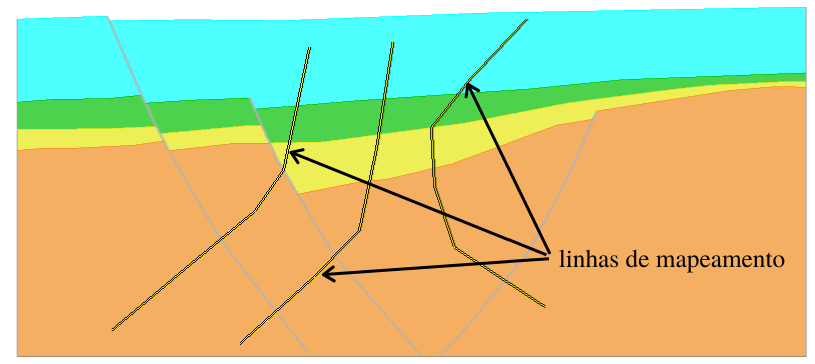
\includegraphics[width=400pt]{images/fig-linhas-de-mapeamento-ed}
    \caption{Linhas de mapeamento em uma seção.}\label{fig-linemap}
  \end{center}
\end{figure}

A Figura~\ref{fig-linemap-history} apresenta o resultado após uma transformação do tipo \textit{Move-Sobre-Falha} onde é possível observar, além da deformação da camada, a linha de mapeamento sofrendo a mesma movimentação. Este tipo de uso pode ser interpretado como se houvesse ali um falso horizonte para avaliar o quantidade de movimento na restauração do rejeito.

\begin{figure} [h]
  \begin{center}
    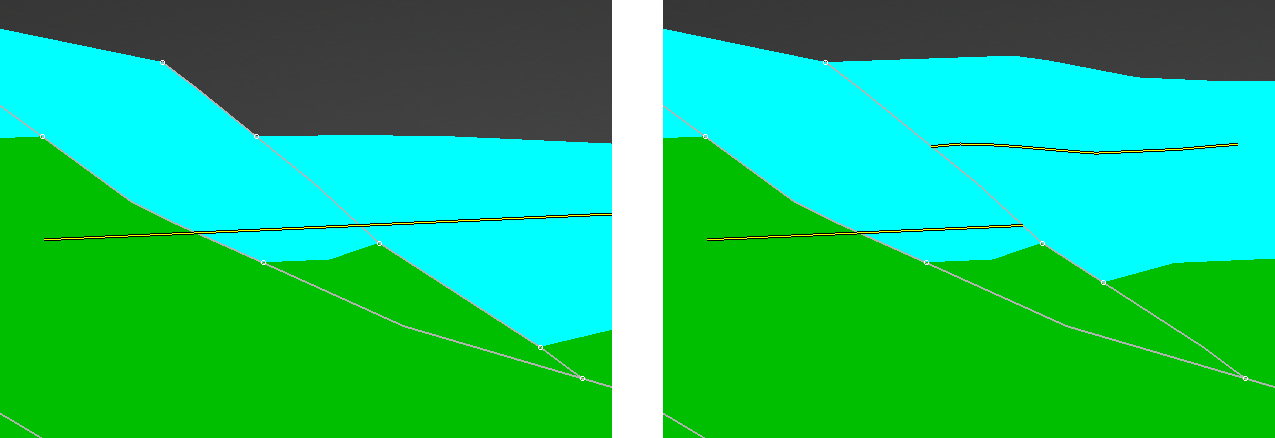
\includegraphics[width=420pt]{images/fig-linemap-history}
    \caption{Linhas de mapeamento em diferentes etapas}\label{fig-linemap-history}
  \end{center}
\end{figure}


O processo de criação da linha de mapeamento é feito para cada parte individualmente, de forma que ao visualizar as partes tem-se a linha de mapeamento completa. Na Figura~\ref{fig-linemap-malhas} é possível ver uma linha de mapeamento cortando algumas regiões diferentes.

\begin{figure} [h]
  \begin{center}
    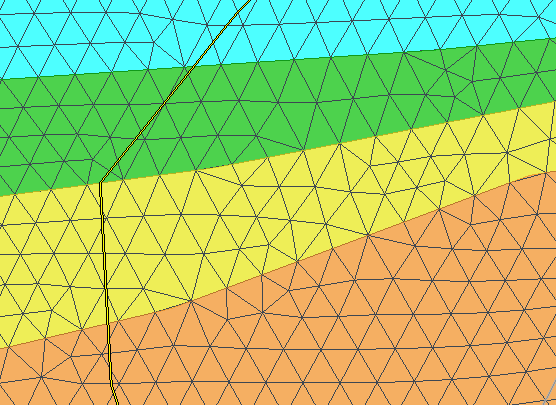
\includegraphics[width=250pt]{images/fig-linhas-de-mapeamento-malhas}
    \caption{Linhas de mapeamento cortando múltiplas faces.}\label{fig-linemap-malhas}
  \end{center}
\end{figure}

Na Figura~\ref{fig-linemap-parts} estão evidenciadas as partes que formam a linha de mapeamento. Como já dito, cada parte está associada à malha de um região diferente.

\begin{figure} [h]
  \begin{center}
    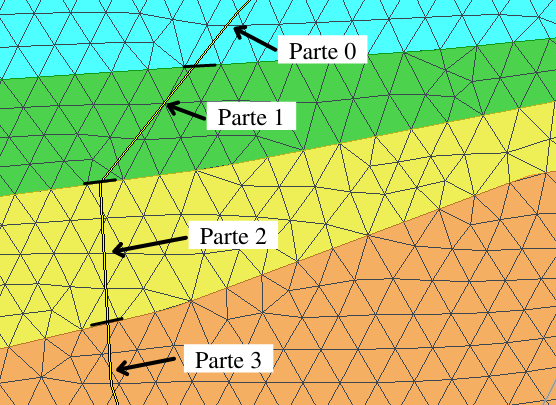
\includegraphics[width=250pt]{images/fig-lm-parts}
    \caption{Partes de uma linha de mapeamento}\label{fig-linemap-parts}
  \end{center}
\end{figure}

A Figura~\ref{fig-lm-topo} mostra a identificação dos pontos em uma parte de linha de mapeamento e a Tabela~\ref{tab-lm-topo} exibe quais informações topológicas são salvas de cada ponto.

\begin{figure} [hbt!]
  \begin{center}
    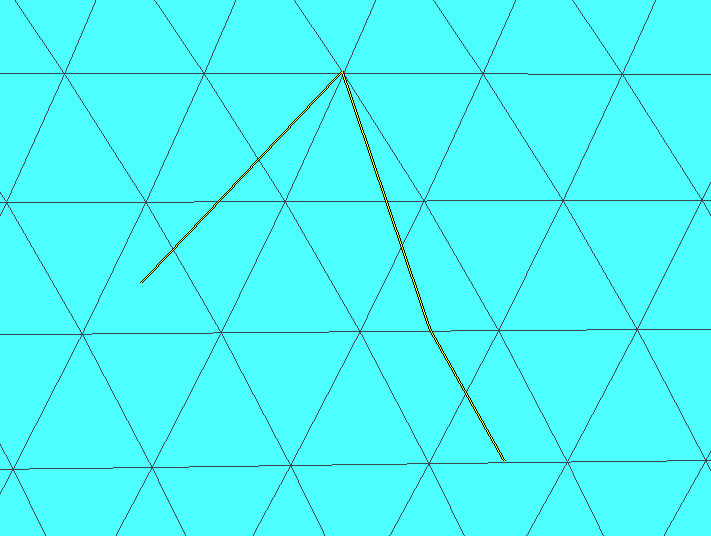
\includegraphics[width=260pt]{images/fig-lm-topo}
    \caption{Informações topológicas da malha mapeadas para a linha de mapeamento.}\label{fig-lm-topo}
  \end{center}
\end{figure}

% -*- coding: utf-8; -*-

\begin{table} [hbt!]
 \begin{center}
	 \caption{Informações topológicas salvas na linha de mapeamento.\label{tab-lm-topo}}
	~\\[-2mm]
	 \begin{tabularx}
		 {\textwidth}
		 {cp{2.0cm} lp{3.0cm} lp{10.0cm}}

		 \textbf{Ponto}
		 & \textbf{Tipo}
		 & \textbf{Informação armazenada} \\ \toprule

		 %~\\[-1mm]
		 A
		 & Elemento
		 & id=30, coordenadas baricêntricas=(0,33; 0,33; 0,33) \\ \midrule

		 %~\\[-1mm]
		 B
		 & Nó   
		 & id=431 \\ \midrule

		 %~\\[-1mm]
		 C
		 & Aresta
		 & id=130, coordenada paramétrica=0,45 \\ \midrule

		 %~\\[-1mm]
		 D
		 & Aresta
		 & id=145, coordenada paramétrica=0,55 \\ \midrule

	 \end{tabularx}
 \end{center}
\end{table}


\section{Derivações das Linhas de Mapeamento}

As linhas de mapeamento têm também casos de usos mais especializados dentro do Sistema Recon, como na criação e representação de poços. Poços são criados semelhantemente às linhas ou por importação de modelos com poços em 3D. Possuem característica de serem linhas quase verticalizadas e possuem uma finalidade mais limitada. Nos casos de poços 3D, a linha correspondente ao poço é apenas uma projeção do objeto tridimensional no plano da seção.

Há o uso nas chamadas linhas de interseção (\textit{CrossLine}) que servem para identificar e mapear as linhas de cruzamento entre seções no espaço tridimensional do multisseções, com isso é possível ter uma noção do que ocorre com seções transversais mesmo estando no domínio bidimensional da restauração.

Por último, foi criada a \textit{linha de mapeamento do modelo} ou \textit{LMModel}, cujo objetivo é servir como um mapeamento das linhas que representam os elementos geológicas ao longo da restauração do modelo. Assim, é possível ter um acompanhamento do que ocorre com as entidades geológicas na seção, além de poder verificar como se deu a movimentação de cada ponto de horizonte, falha ou topo de sal ao longo da restauração.

As \textit{LMModels} são linhas de mapeamento baseadas no pontos do contorno da malha das regiões, ou seja, as partes que a formam possuem apenas pontos de mapeamento do tipo nó.

Pelo objetivo proposto, as \textit{LMModels} são linhas de mapeamento que tomam a geometria das entidades geológicas como entrada, então não há necessidade de criar uma linha-guia como é feita na linha de mapeamento original, a própria linha de horizonte, falha, ou topo de sal é usada como linha-guia.

Conforme o elemento geológico base, há um tipo de \textit{LMModel} e informações adicionais armazenadas:

\renewcommand{\labelitemi}{•}
\begin{itemize}
  \item Horizonte: é guardado a informação de idade deste horizonte.
  \item Falha: o identificador da falha é o dado armazenado.
  \item Topo de sal: apenas uma referência direta à linha original.
\end{itemize}

Todas essas informações  geológicas atreladas ao mapeamento topológico das \textit{LMModels}, quando em conjunto com as diversas seções geológicas de um modelo multisseções, são o que fazem dela o principal dado para a realização de um mapeamento de informações de evolução do modelo tridimensional ao longo do tempo, já que trazem todo o histórico de movimentação das camadas de um modelo geológico.

A maneira de trabalhar com \textit{LMModels} é com a organização delas em estruturas de dados que formam subconjuntos divididos por etapa de restauração e idade (caso de linhas de horizonte), o que será visto adiante. Com isso é obtido o conjunto de informações que representam a restauração das seções no Sistema Recon.

\begin{figure} [h]
  \begin{center}
    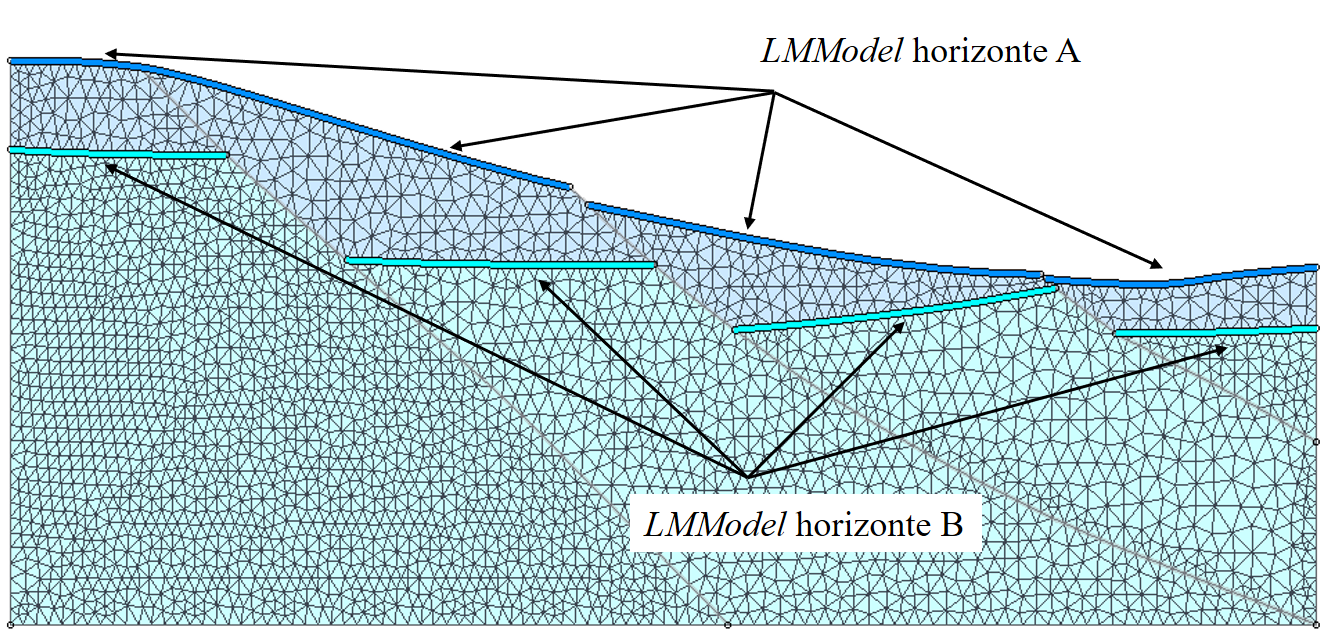
\includegraphics[width=350pt]{images/fig-lmmodel-example}
    \caption{\textit{LMModels} em uma seção geológica no Sistema Recon}\label{fig-lmmodel-example}
  \end{center}
\end{figure}

A Figura~\ref{fig-lmmodel-example} mostra \textit{LMModels} de dois horizontes diferentes. A representação delas dentro do Sistema Recon é feita com uma linha de maior espessura que as linhas de horizonte, no entanto, os pontos são os mesmos do contorno da malha. Perceba na Figura~\ref{fig-lmmodel-mesh-diff} a diferença entre a linha de horizonte e a \textit{LMModel}, evidenciando o contorno da malha entre as duas regiões.

\begin{figure} [h!]
  \begin{center}
    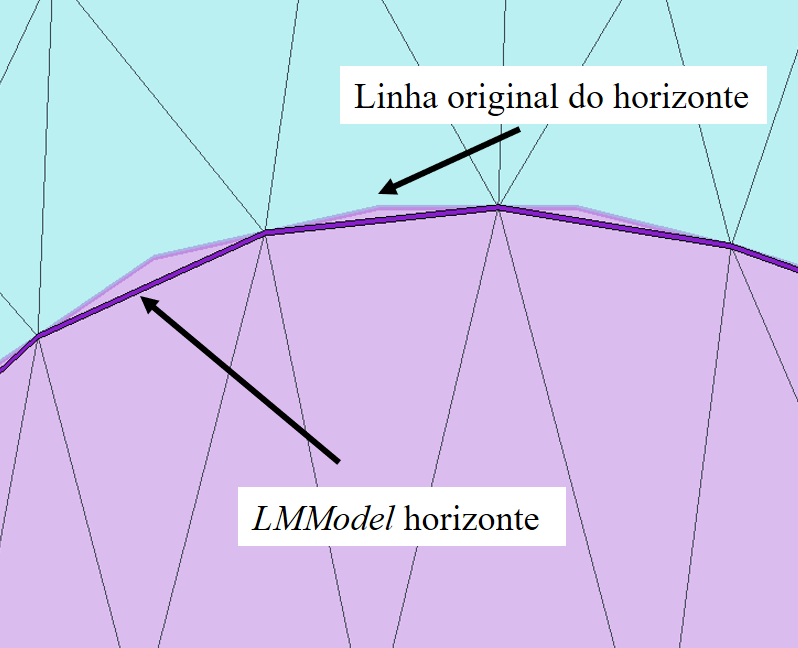
\includegraphics[width=275pt]{images/fig-lmmodel-mesh-diff}
    \caption{Diferença entre \textit{LMModel} e a linha de horizonte e uma seção geológica no Sistema Recon}\label{fig-lmmodel-mesh-diff}
  \end{center}
\end{figure}

A próxima ilustração na Figura~\ref{fig-lmmodel-ms} apresenta as \textit{LMModels} de dois horizontes em um modelo multisseções. É esse conjunto de informações no ambiente tridimensional que será usado como parâmetro para o mapeamento de superfícies no Sistema Recon.

\begin{figure} [h!]
  \begin{center}
    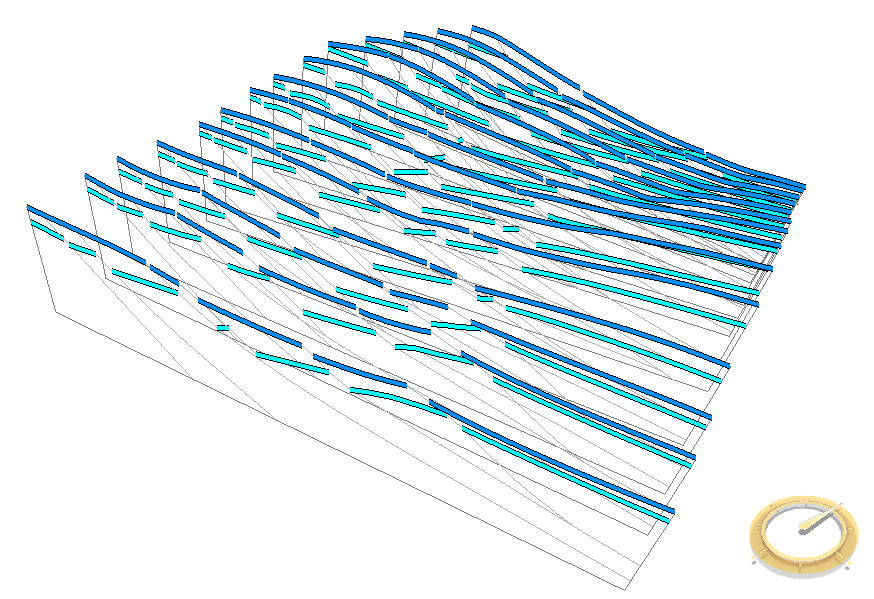
\includegraphics[width=300pt]{images/fig-lmmodel-ms}
    \caption{\textit{LMModels} no ambiente multisseções do Sistema Recon}\label{fig-lmmodel-ms}
  \end{center}
\end{figure}

\section{Mapeamento de superfícies}

\subsection{Metodologia}

Na seção anterior foi apresentado um tipo de mapeamento bidimensional que é usado dentro da restauração de seções do Sistema Recon. Aqui será mostrado o mapeamento de superfícies que, neste trabalho, pode ser definido como o uso de informações das seções como parâmetros matemáticos para deformar os pontos da superfície e assim obter uma configuração coerente com a movimentação tectônica resultante da restauração das seções geológicas. A metodologia a seguir foi apresentada por Müller\cite{Muller} para tratar a deformação de superfícies com o uso de restrições presentes no domínio da mesma e através de minimização de uma energia.

A deformação de uma superfície pode ser modelada como um problema variacional em termos de energia através de funções Lagrangeanas que por sua vez podem ser descritas pelo operador de Laplace com diferentes ordens. A energia de superfície de membrana é uma PDE de segunda ordem, descrita pelo operador de Laplace $\Delta{q}$ e minimiza a área da superfície. A energia de placas-finas que minimiza a curvatura da superfície é descrita pela PDE de quarta ordem $\Delta^2{q}$. Já para minimização da variação da curvatura de superfícies pode ser usada uma PDE de sexta ordem, ou tri-harmônica, $\Delta^3{q}$, sua aproximação discreta é dita superfície de mínima variação.\cite{Muller, Botsch}

Essa deformação pode ocorrer com base em duas premissas: que sejam conhecidas a posição inicial dos pontos da superfície e a posição deformada de pontos de controle (que também pertencem à superfície). A partir da informação desses pontos de controle busca-se encontrar a posição deformada de todos os pontos da superfície. A solução desse problema começa na obtenção de uma solução estacionária que minimize uma energia.\cite{Muller}

Dois tipo de métodos podem ser usados para, dada uma superfície $\mathcal{S}$ num espaço $R^3$ com contorno $\Omega$ descrita num espaço cartesiano $x$ com pontos iniciais conhecidos e pontos de controle cujas deformações são conhecidas, calcular a deformação de $\mathcal{S}$. Os métodos baseados em superfície que dependem de uma boa qualidade da representação discreta da superfície e os baseados em deformação espacial que, como diz o nome, não dependem da representação da superfície.\cite{Botsch} Dentre este últimos, cita-se: 

\renewcommand{\labelitemi}{•}
\begin{itemize}
  \item o método Lattice Based Freeform Deformation que usa funções de forma B-spline e um tensor descrito pelos pontos de controle, sua formulação resulta em um sistema retangular de equações lineares solucionável por meio de inversas generalizadas ou mínimos quadrados;
  \item o método Cage Based Freeform Deformation que pode ser considerado uma generalização do método anterior e utiliza uma gaiola de malha grossa que engloba a superfície a ser deformada e uma interpolação linear entre os pontos da gaiola e os pontos de controle que por sua vez compõem novas funções de interpolação;
  \item o método com Radial Basis Functions (RBF), conhecido por interpolar muito bem dados de nuvens de pontos e será visto em mais detalhes a seguir.
\end{itemize}

Considere $m$ conhecidos pontos de controle $\boldsymbol{s}=\{s_1, s_2, \ldots, s_m\}$ e outros $n$ pontos com posição final desconhecidas $\boldsymbol{v}=\{v_1, v_2, \ldots, v_n\}$ de uma superfície $\mathcal{S}$, sendo conhecida a posição deformada dos $m$ pontos $\boldsymbol{s'}=\{s'_1, s'_2, \ldots, s'_m\}$ em $\mathcal{S}'$, precisamos definir uma função $\boldsymbol{d}\to R^3$ que interpole exatamente os $m$ pontos $\boldsymbol{d}(s_i)=(s'_i-s_i)$ e que interpole, garantindo a solução estacionária da função Lagrangeana, os $n$ pontos desconhecidos.

Uma RBF é representada pela combinação linear de kernels radialmente simétricos $\varphi_j(\boldsymbol{x})=\lVert\boldsymbol{x}_j-\boldsymbol{x}\rVert$ localizados nos centros $\boldsymbol{x}_j\subset R^3$ ponderados por funções peso $\boldsymbol{w}_j\subset R^3$ somada a um polinômio de baixo grau (cuja base é $\pi(\boldsymbol{x})=\{x,y,z,1\}$ e ponderado por $\boldsymbol{\lambda}_k\subset R^3$) para garantir precisão polinomial:

\begin{align}
  &\boldsymbol{d}(x)=\sum_{j=1}^m \boldsymbol{w}_j\varphi_j(\boldsymbol{x})+\sum_{k=1}^4 \boldsymbol{\lambda}_k\pi_k(\boldsymbol{x})\label{eq-surf-rbf}
\end{align}

De volta ao início do problema, o interesse é solucionar a PDE tri-harmônica $\Delta^3\boldsymbol{d}(x)=0$, para isso é preciso escolher uma função kernel que seja solução fundamental dessa equação. Foi mostrado por Botsch\cite{Botsch} que $\varphi(r)=r^3$ é uma solução fundamental que leva para uma superfície de variação mínima. Para solução baseada em superfície, essa minimização deve ser obtida de forma explícita. Os coeficientes $\boldsymbol{w}_j$ e $\boldsymbol{\lambda}_k$ são obtidos com a solução de um sistema linear (Eq.~\ref{eq-ls-surf-deformer}) de equações $(m+4)\times(m+4)$ desde que se satisfaça a interpolação dos $m$ pontos de controle com as restrições impostas nas posições $x_j=s_j$.\cite{Muller}

\begin{align}
  \begin{bmatrix}
    \varphi_1(s_1) & \cdots & \varphi_m(s_1) & \pi_1(s_1) & \cdots & \pi_4(s_1)\\ 
    \vdots & \ddots & \vdots & \vdots & \ddots & \vdots\\
    \varphi_1(s_m) & \cdots & \varphi_m(s_m) & \pi_1(s_m) & \cdots & \pi_4(s_m)\\ 
    \pi_1(s_1) & \cdots & \pi_1(s_m) & 0 & \cdots & 0\\
    \vdots & \ddots & \vdots & \vdots & \ddots & \vdots\\
    \pi_4(s_1) & \cdots & \pi_4(s_m) & 0 & \cdots & 0
  \end{bmatrix}
  \begin{Bmatrix}
    w_1^T\\
    \vdots\\
    w_m^T\\
    \lambda_1^T\\
    \vdots\\
    \lambda_4^T
  \end{Bmatrix}=
  \begin{Bmatrix}
    (s'_1-s_1)^T\\
    \vdots\\
    (s'_m-s_m)^T\\
    0\\
    \vdots\\
    0
  \end{Bmatrix}\label{eq-ls-surf-deformer}
\end{align}

Depois de resolver o sistema de equações e conseguir os coeficientes de ponderação, os $n$ pontos desconhecidos podem ser obtidos com $v'_i=v_i+\boldsymbol{d}(v_i)$.

A fim de demonstrar as diferenças para diferentes tipos de energias para a função Lagrangeana na deformação de uma superfície, é apresentado o exemplo a seguir, Figura~\ref{fig-eg-surf-deformer-1}. Uma superfície quadrada e plana de comprimento $L=20m$,com seu contorno deformado da seguinte forma: topo e base segundo uma função senoidal $z_{y(0,L)}=\frac{L}{2}\sin(\frac{\pi x}{L})$ e laterais fixas. Os resultados obtidos levaram em consideração as Lagrangeanas de segunda ordem $\Delta\boldsymbol{d}=0$, quarta ordem $\Delta^2\boldsymbol{d}=0$ e sexta ordem $\Delta^3\boldsymbol{d}=0$.

\begin{figure} [H]
  \begin{center}
    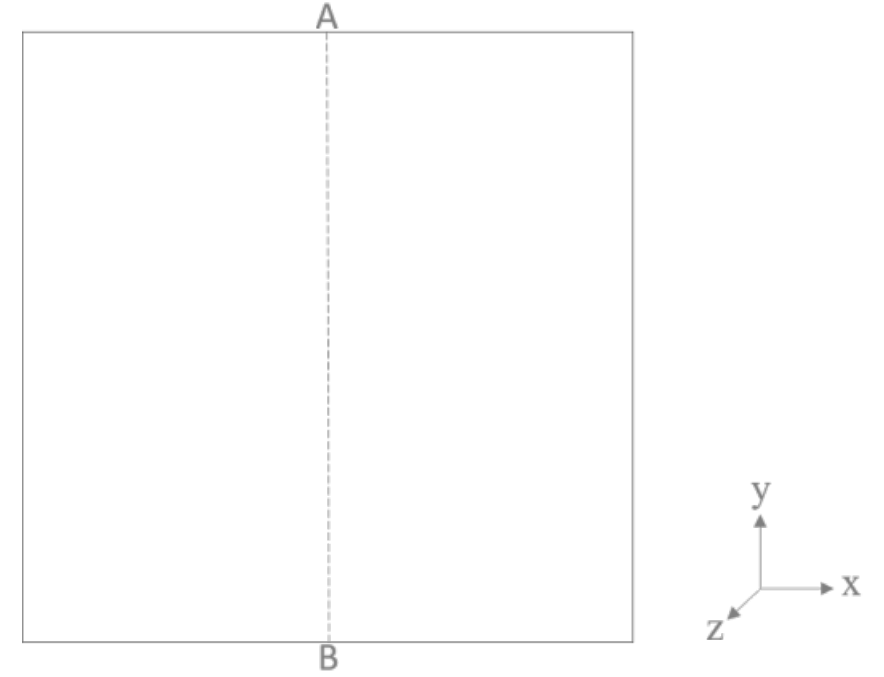
\includegraphics[width=200pt]{images/fig-eg-surf-deformer-1}
    \caption{Configuração inicial da superfície a ser deformada.\cite{Muller}}\label{fig-eg-surf-deformer-1}
  \end{center}
\end{figure}


\begin{figure} [H]
  \begin{center}
    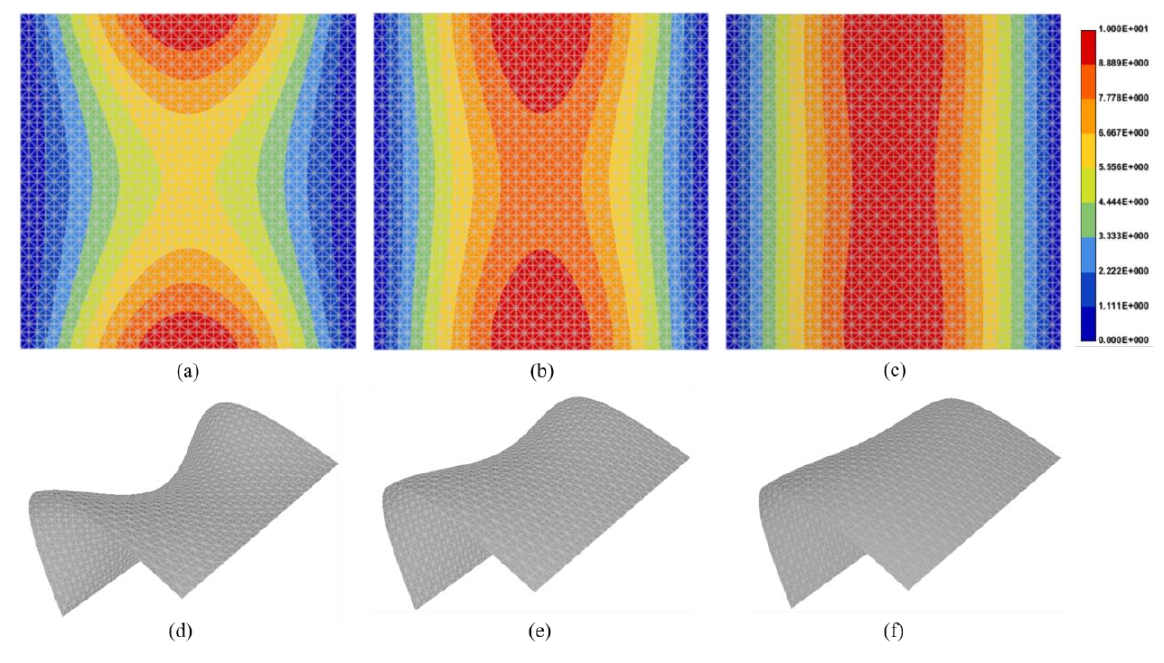
\includegraphics[width=\textwidth]{images/fig-eg-surf-deformer-2}
    \caption{Configuração deformada da superfície segundo as Lagrangeanas de 2ª ordem (a,d), 4ª ordem (b,e) e 6ª ordem (c, f). As figuras (a, b e c) representam os resultados na direção $z$, escala em metros.\cite{Muller}}\label{fig-eg-surf-deformer-2}
  \end{center}
\end{figure}

A Figura~\ref{fig-eg-surf-deformer-2} deixa clara as diferenças na deformação da superfície conforme a energia minimizada. De modo específico para a deformação de superfícies geológicas onde há um viés físico atrelado, a solução que minimiza a energia de mínima variação e que, portanto, resulta na mínima variação da curvatura é a que melhor se adequa ao comportamento previsto para este tipo de simulação.

O gráfico da Figura~\ref{fig-eg-surf-deformer-3} a seguir destaca o campo de deslocamentos em $z$ sobre o segmento $\overline{AB}$ da Figura~\ref{fig-eg-surf-deformer-1} para cada um dos tipos de deformação obtida.

\begin{figure} [H]
  \begin{center}
    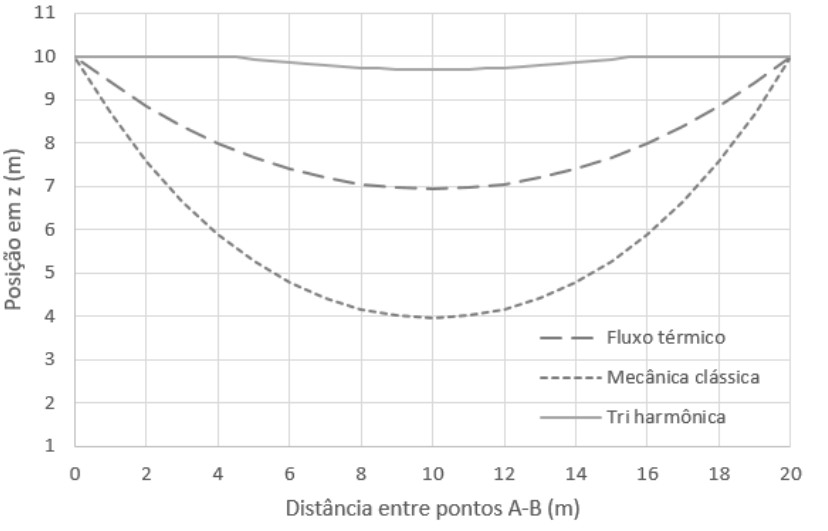
\includegraphics[width=250pt]{images/fig-eg-surf-deformer-3}
    \caption{Coordenada $z$ sobre o segmento $\overline{AB}$.\cite{Muller}}\label{fig-eg-surf-deformer-3}
  \end{center}
\end{figure}

\subsection{Preparação dos dados}

% Dados
% É preciso que o modelo esteja com as seções restauradas
% Modelo precisa estar dividido em etapas
% As superfícies precisam estar com as lmmodels na malha
 
A metodologia mostrada anteriormente é capaz de realizar a deformação de superfície mediante conhecimento da posição inicial da mesma e também de informação de movimentação de pontos de controle, pontos estes que devem fazer parte do domínio da superfície. Desse modo, no contexto de restauração de seções no Sistema Recon, o mapeamento de superfície é obtido com a deformação desta superfície de acordo com parâmetros provenientes das seções, em outras palavras, o mapeamento de superfície usa dados das seções como pontos de controle para se conseguir um comportamento equivalente no ambiente tridimensional. Essa é forma sucinta de dizer a maneira como o o mapeamento de superfície é feito. Nesta subseção serão apresentadas as etapas que permitem o uso do deformador de superfícies com o intuito de se obter o mapeamento de superfícies.

\subsubsection{\textit{LMModels}}

O objetivo aqui é mostrar como obter informação de deslocamento dos horizontes entre etapas de restauração de uma seção a partir de \textit{LMModels}. Esse deslocamento é o dado principal vindo das seções para o mapeamento de superfície, o deslocamento de pontos de horizonte; horizontes estes que coincidem com a superfície tridimensional, uma vez que as seções geológicas são cortes transversais planos de um conjunto de superfícies tridimensionais.

Como já visto, as \textit{LMModels} são linhas de mapeamento da seção baseadas em entidades geológicas. Estas linhas acompanham a movimentação tectônica na seção durante a restauração. Para esta etapa do trabalho, considerar-se-á apenas as \textit{LMModels} de horizonte, ou seja, aquelas que tem como origem uma linha de horizonte, como as mostradas na Figura~\ref{fig-lmm-horizons}.

\begin{figure} [H]
  \begin{center}
    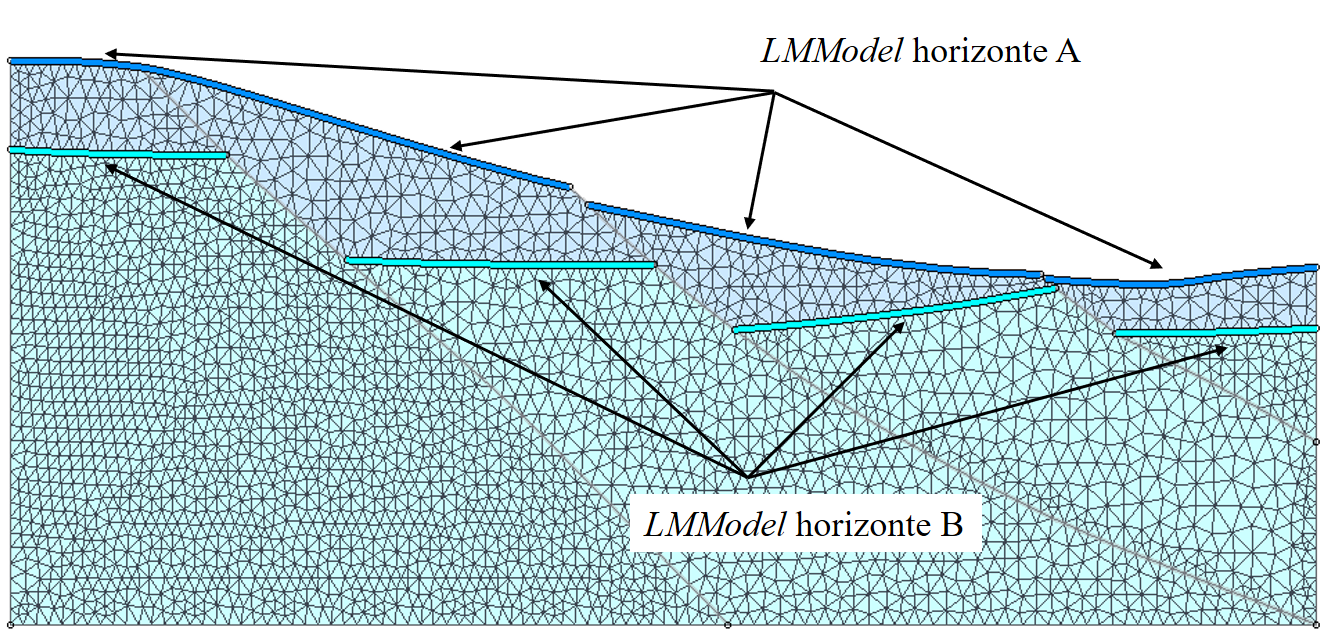
\includegraphics[width=350pt]{images/fig-lmmodel-example}
    \caption{\textit{LMModels} de horizonte no Sistema Recon}\label{fig-lmm-horizons}
  \end{center}
\end{figure}

A movimentação tectônica da seção pode ser mensurada como uma diferença entre uma e outra etapa de restauração, mais especificamente, a distância entre os pontos de \textit{LMModels} correspondentes entre a etapa atual e a próxima.

A \textit{LMModel} em si não possui pontos geométricos, ela armazena apenas os índices dos nós do contorno da malha na extensão correspondente a uma linha de horizonte (Figura~\ref{fig-lmm-mesh-boundary}), dessa forma, entre um cenário e outro da mesma seção, pode ocorrer uma edição na malha que pode alterar os nós do contorno e assim alterando o conjunto de índices que formam a \textit{LMModel}.

\begin{figure} [H]
  \begin{center}
    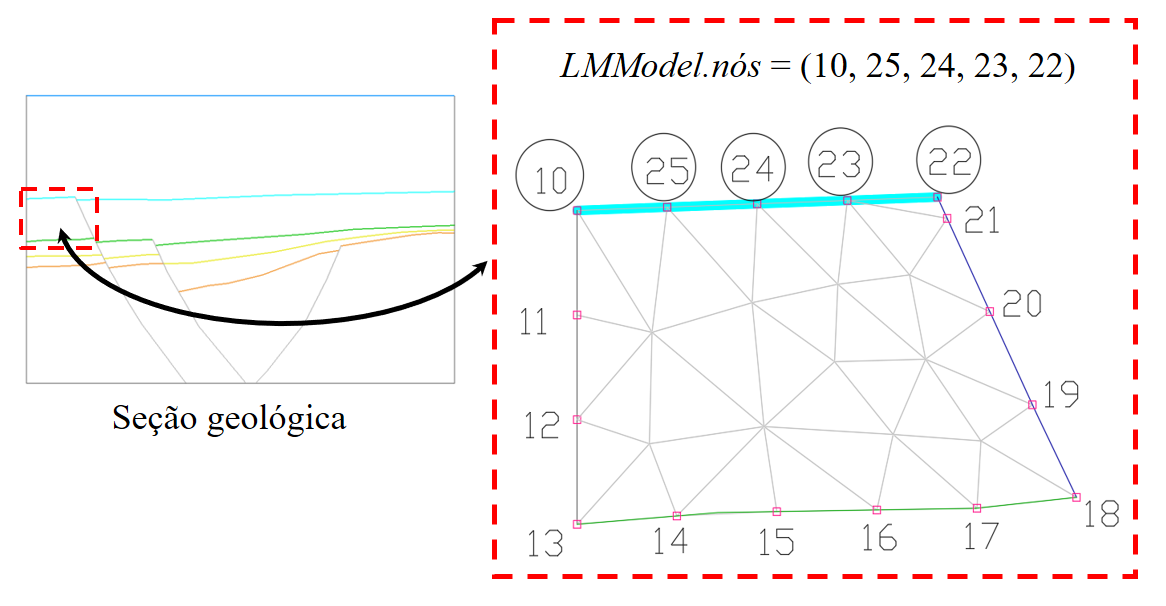
\includegraphics[width=310pt]{images/fig-lmm-mesh-boundary}
    \caption{Índices de nós que compõem uma parte de \textit{LMModels}.}\label{fig-lmm-mesh-boundary}
  \end{center}
\end{figure}

Para que se faça uma relação direta de deslocamento entre pontos de uma \textit{LMModel} em um e outro cenário é necessário que se faça uma interpolação entre as malhas envolvidas. Esta ação serve para assegurar que se tenha um mesmo número de pontos formando a \textit{LMModel} correspondente ao longo da restauração de uma seção.

Para exemplificar melhor este problema, considere a seção geológica da Figura~\ref{fig-lmm-interp1} (a) que destaca os pontos que formam a \textit{LMModel} do horizonte A (do topo). Considera-se que na etapa seguinte (cenário 2), houve uma transformação e uma edição na malha, com isso a \textit{LMModel} correspondente teve diminuição no número de pontos, como mostra a Figura~\ref{fig-lmm-interp1} (b).

\begin{figure} [H]
  \begin{center}
    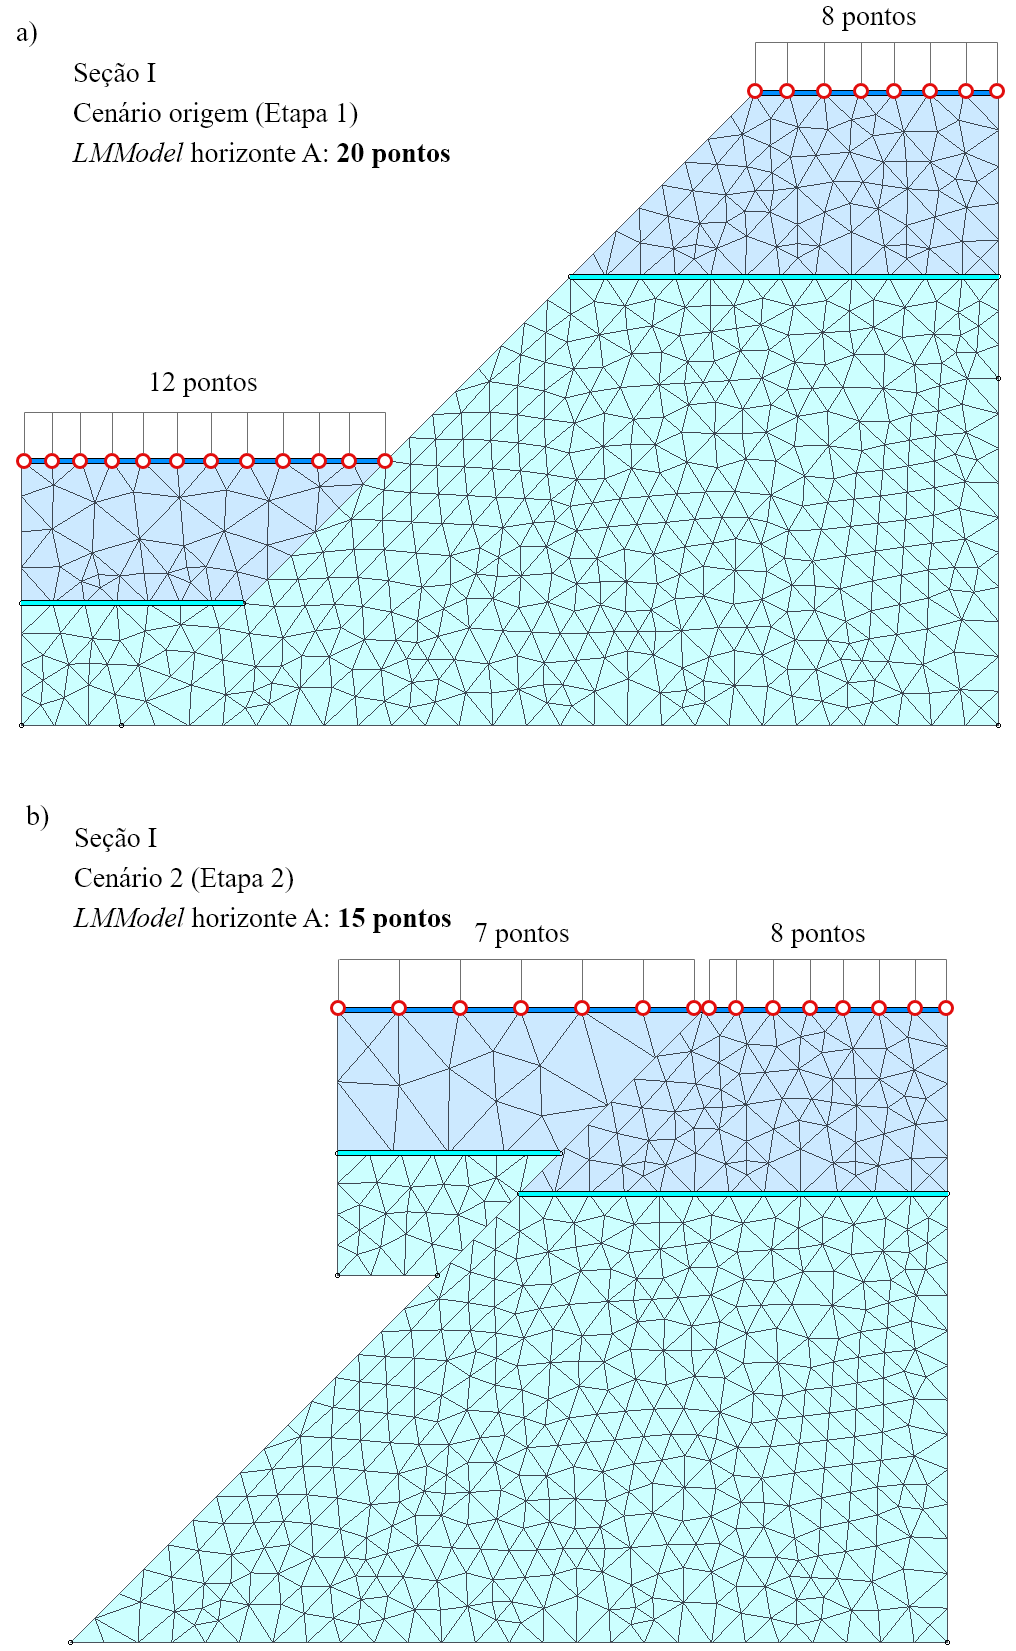
\includegraphics[width=300pt]{images/fig-lmm-interp1}
    \caption{\textit{LMModel} no cenário origem e cenário 2 com diferente número de pontos.}\label{fig-lmm-interp1}
  \end{center}
\end{figure}

Para que seja feito o cálculo de deslocamento entre as \textit{LMModels} destes cenários é necessário uma interpolação entre as malhas, como já dito. Essa interpolação vai dizer quais os pontos da \textit{LMModel} do cenário origem correspondem no cenário 2 e assim ter dados para encontrar informações de deslocamento de uma etapa a outra.

Convencionou-se neste trabalho que a obtenção dos pontos de \textit{LMModels} tomará como base para interpolação aquela criada no cenário origem, já que é um cenário mais restrito para edições após o início da restauração, além de um outro motivo que será apresentado adiante. Um esquema mais explicativo é visto na Figura~\ref{fig-lmm-interp2}.

\begin{figure} [H]
  \begin{center}
    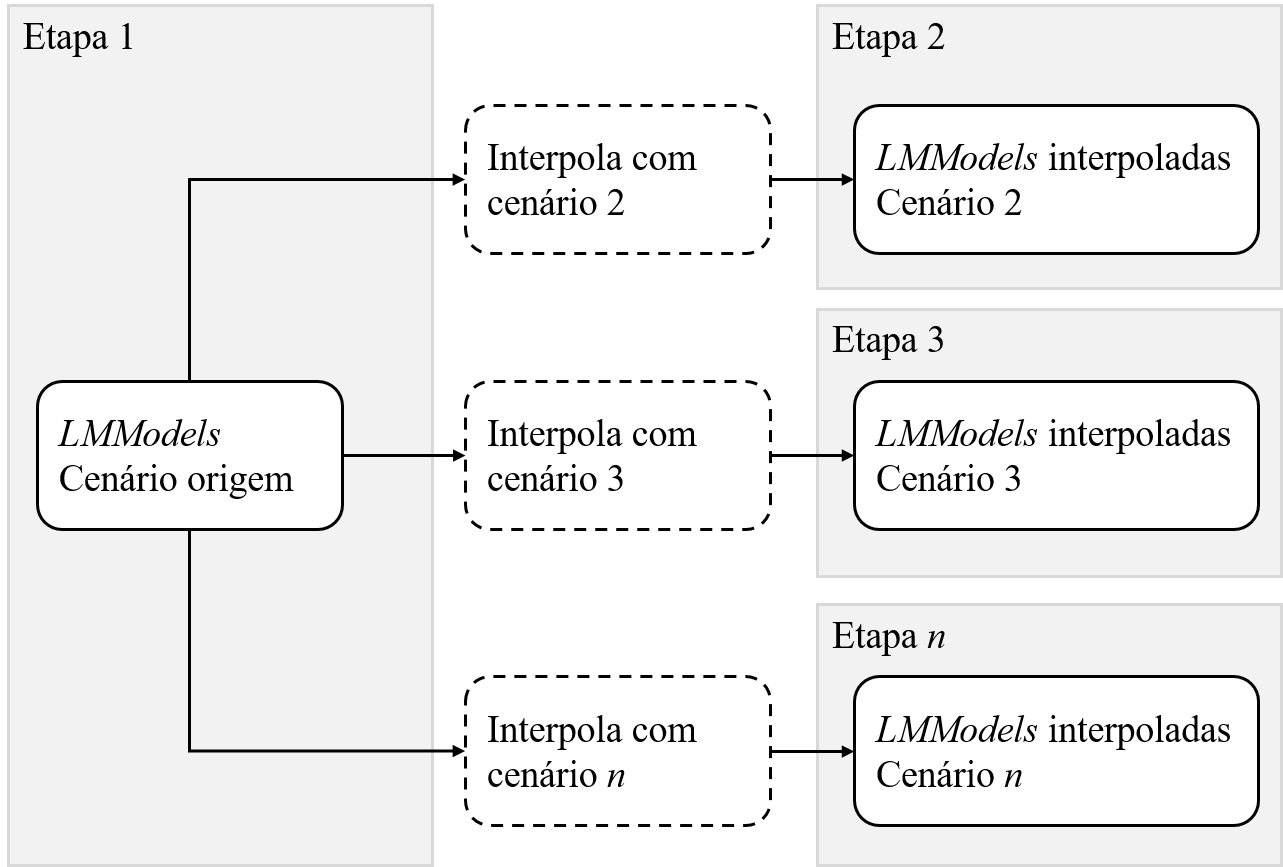
\includegraphics[width=350pt]{images/fig-lmm-interp2}
    \caption{Esquema de como obter número igual de pontos de \textit{LMModels} em diferentes cenários}\label{fig-lmm-interp2}
  \end{center}
\end{figure}

Ao se repetir esta ação para todas as seções que compõem o modelo, é possível criar uma estrutura de dados multidimensional com todos os pontos geométricos que formam as \textit{LMModels} a fim de facilitar o uso dessas informações. De maneira sucinta esta estrutura é apresentada na Figura~\ref{fig-lmm-data-structure} como sendo análoga a uma matriz de 3 dimensões e cada elemento é um conjunto de dois pontos cartesianos\footnote{os pontos nas malhas da seção estão em coordenadas bidimensionais, no entanto, ao criar esta estrutura de dados, todos os pontos são convertidos para coordenadas espaciais \textit{x}, \textit{y} e \textit{z} com base nas coordenadas UTM onde a seção se localiza.} e um dado booleano que indica se houve movimentação quando a diferença entre os pontos \textit{current} e \textit{next} é maior que uma dada tolerância.

\begin{figure} [H]
  \begin{center}
    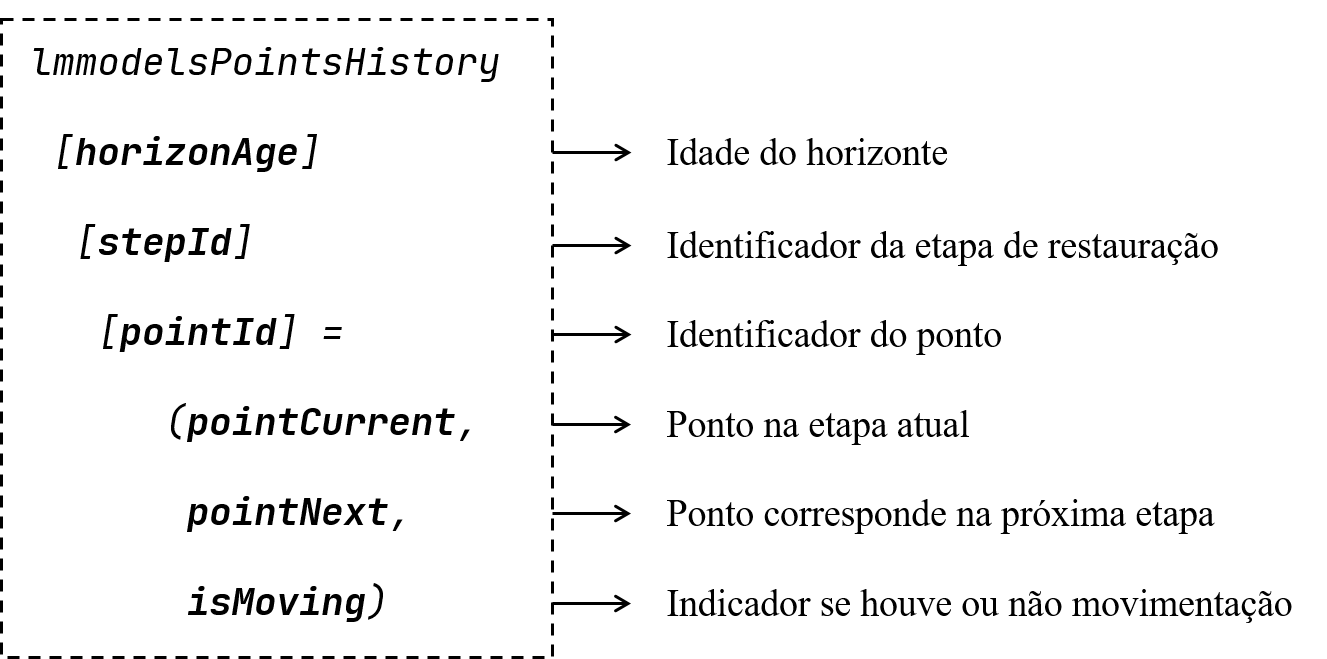
\includegraphics[width=350pt]{images/fig-lmm-data-structure}
    \caption{Estrutura de dados que armazena os pontos das \textit{LMModels} do modelo.}\label{fig-lmm-data-structure}
  \end{center}
\end{figure}

Outra informação importante é que deve se ter o modelo já com todas as seções restauradas, uma vez que qualquer edição posterior nas seções, acarretará na necessidade de recriar a estrutura de dados de \textit{LMModels}.

\subsubsection{\textit{Remesh} da superfície}

Na parte sobre a metodologia do deformador de superfície, apresentada anteriormente, é apontado a necessidade de haver pontos de controle pertencentes à superfície, pontos estes que precisam ter sua posição final conhecida. Pois bem, uma parte destes pontos de controle são as \textit{LMModels}, ou melhor, os pontos que representam o histórico de movimentação das \textit{LMModels}.

A interseção de um plano transversal a um conjunto de superfícies geológicas tridimensionais é o que produz a seção geológica, onde cada linha de horizonte é a representação de uma parte da superfície no plano bidimensional. Não por acaso, as \textit{LMModels} são mapeamentos dessas linhas de horizonte e, portanto, também mapeiam a superfície. No entanto, os pontos que formam a \textit{LMModel} foram gerados com base nas malhas de triângulos da seção e não possuem qualquer relação com os pontos que estão na superfície.

Com a finalidade de resolver esse problema é apresentado nesta subseção a necessidade de um \textit{remesh} (regeração) da malha que forma a superfície, cujo objetivo é produzir uma nova que contenha os pontos que formam as \textit{LMModels} das seções geológicas.

O \textit{remesh} é realizado com auxílio do algoritmo de regeração de malhas de superfícies considerando curvaturas proposto por Miranda \textit{et al.}\cite{Miranda}. Os dados de entrada são as linhas de borda da superfície e uma superfície de suporte representada por três funções generalizadas, criadas a partir da superfície de suporte:

\renewcommand{\labelitemi}{•}
\begin{itemize}
  \item 1ª função: recebe um ponto da superfície como entrada e devolve o tamanho característico da aresta de um triângulo equilátero ideal na posição desse ponto. O cálculo desse tamanho envolve o uso de uma estrutura de dados \textit{octree}\footnote{Uma estrutura de árvore onde cada nó pode possuir oito filhos e representa a subdivisão do espaço em oito octantes\cite{Donald}.} que fornece um refinamento de tamanho de acordo com a curvatura da superfície.
  \item 2ª função: calcula o ponto ideal que irá formar um novo triângulo de acordo com uma dada aresta no processo de contração de contorno de geração da malha. Além da aresta, são passados a função a altura do triângulo e um vetor unitário na direção perpendicular à aresta que será usado para definir o plano de interseção com a superfície e assim encontrar o ponto ideal.
  \item 3ª função: usada para melhoria na malha após a suavização. Recebe um ponto qualquer e retorna o ponto mais próximo pertencente à malha da superfície de suporte. Com a suavização, alguns nós mudam de lugar e podem acabar fora da superfície, aí entra o uso desta função para trazer de volta os pontos distantes. 
\end{itemize}

O algoritmo utiliza avanço de fronteira na primeira fase e faz uso da 1ª e 2ª funções para determinar a primeira versão da nova malha. Após isso começa a etapa de melhoria com suavização e em paralelo, o uso da 3ª função\cite{Miranda}. O resultado final é uma malha com elementos melhor discretizados em regiões de alta curvatura, como mostra a Figura~\ref{fig-remesh} onde as imagens (a) e (b) são as superfícies de suporte e as imagens (c) e (d) suas versões regeradas, respectivamente.

\begin{figure} [H]
  \begin{center}
    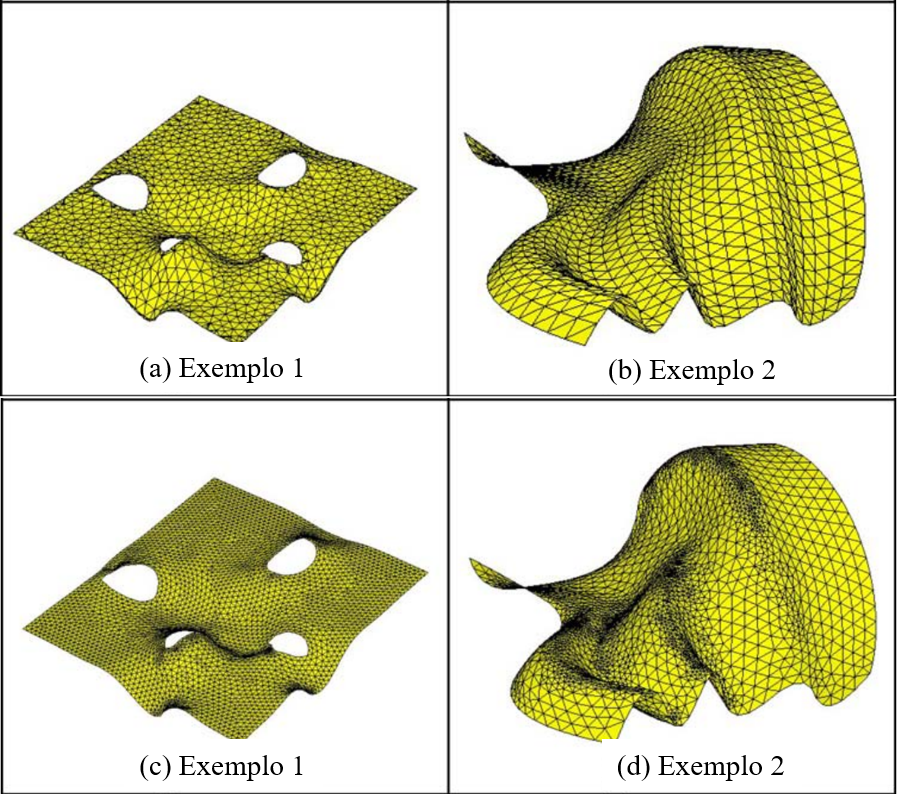
\includegraphics[width=350pt]{images/fig-remesh}
    \caption{Exemplo de resultado obtido com algoritmo de \textit{remesh}\cite{Miranda}.}\label{fig-remesh}
  \end{center}
\end{figure}

\subsubsection{Coleta bordas origem/destino}


\subsubsection{Definição de movimentação das amostras}


\subsection{Exemplos e resultados}

\section{Mapeamento do Volume}

\subsection{Metodologia}

\subsection{Preparação dos dados}

\subsection{Exemplos e resultados}


